% Report title macro for consistent headers
\newcommand{\ReportTitle}{Wibe Crawler: An AI-Powered Autonomous Penetration Testing System}

% !TEX root = wibe-crawler-report.tex

\documentclass[12pt,oneside,a4paper]{book}

% Packages
\usepackage[utf8]{inputenc}
\usepackage{graphicx}
\usepackage{fancyhdr}
\usepackage{amsmath, amssymb}
\usepackage{setspace}
\usepackage{float}
\usepackage[left=1.35in, right=1.35in, bottom=1in, includefoot]{geometry}
\usepackage{ragged2e}
\usepackage{enumitem}
\usepackage{comment}
\usepackage{array}
\usepackage{xcolor}
\definecolor{lightgrey}{gray}{0.95}
\definecolor{darkgrey}{gray}{0.3}
\usepackage{subcaption}
\usepackage[labelfont=bf]{caption}
% Always include figures in List of Figures
\captionsetup[figure]{list=true}
\usepackage[titletoc]{appendix}
\usepackage{titlesec}
\usepackage{newtxtext,newtxmath}
\usepackage{booktabs}
\usepackage{hyperref}

% TikZ for diagrams
\usepackage{tikz}
\usetikzlibrary{arrows.meta,positioning,fit,shapes.geometric,shadows}
\usepackage{pgfplots}

% Table layout helpers
\usepackage{tabularx}
\renewcommand{\arraystretch}{1.2}

% Page Setup (match template styling)
\onehalfspacing
\setlength{\headheight}{15pt}

% Chapter/Section styling similar to template
\titleformat{\chapter}[display]
  {\normalfont\large\bfseries\centering}
  {\chaptertitlename\ \thechapter}
  {7pt}
  {\MakeUppercase}

\titleformat{\section}
  {\normalfont\bfseries\raggedright}
  {\thesection}
  {1em}
  {\MakeUppercase}

\titleformat{\subsection}
  {\normalfont\bfseries\raggedright}
  {\thesubsection}
  {1em}
  {}

\titleformat{\subsubsection}
  {\normalfont\bfseries\itshape\raggedright}
  {\thesubsubsection}
  {1em}
  {}

% Default fancy page style with report title in header
\pagestyle{fancy}
\fancyhf{}
\fancyhead[L]{{\it\footnotesize \ReportTitle}}
\fancyhead[R]{\bf \thepage}
\fancyfoot[L]{{\it Department of CC}}
\fancyfoot[R]{\it\footnotesize St. Joseph's College of Engineering \& Technology, Palai}
\renewcommand{\headrulewidth}{1pt}
\renewcommand{\footrulewidth}{0.5pt}

% Ensure 'plain' pages (chapter starts, etc.) use the same header/footer
\fancypagestyle{plain}{%
  \fancyhf{}
  \fancyhead[L]{{\it\footnotesize \ReportTitle}}
  \fancyhead[R]{\bf \thepage}
  \fancyfoot[L]{{\it Department of CC}}
  \fancyfoot[R]{\it\footnotesize St. Joseph's College of Engineering \& Technology, Palai}
  \renewcommand{\headrulewidth}{1pt}
  \renewcommand{\footrulewidth}{0.5pt}
}

% Table format
\newcolumntype{C}{>{\centering\arraybackslash}m{3cm}}

\begin{document}

% ---------------- Title Page ----------------
\pagestyle{empty}

\begin{titlepage}
    \begin{center}
      \setlength{\baselineskip}{.75cm}
      
      {\fontsize{16pt}{19.2pt}\selectfont  \bfseries \MakeUppercase {WIBE CRAWLER: AN AI-POWERED AUTONOMOUS PENETRATION TESTING SYSTEM.}}\\[1cm]
      {\large \bf Project Report}\\[1cm]

      {\normalsize \it Submitted in partial fulfillment of the requirements for the award of the degree of}\\[0.5cm]
      {\large \bf Bachelor of Technology}\\
      {\normalsize \it in}\\
      {\large \bf Computer Science and Engineering (Cyber Security)}\\
      \vspace{0.5cm}
      {\large \it Submitted by}\\[0.5cm]
      {\large \textbf{AJAY VARMA J} (Reg.No: SJC22CC004)}\\
      {\large \textbf{ALVIN VARGHESE GEORGE} (Reg.No: SJC22CC012)}\\
      {\large \textbf{MILAN SUMAN} (Reg.No: SJC22CC041)}\\
      {\large \textbf{MUHAMMAD ASLAM A} (Reg.No: SJC22CC042)}\\[2cm]
      \includegraphics[width=1.2in]{sjcet.png}\\[0.5cm]
      \centerline {\large \textbf{Department of Computer Science and Engineering (Cyber Security)}}
      \vspace{.25cm}
      \centerline {\large \textbf{ST. JOSEPH'S COLLEGE OF ENGINEERING AND TECHNOLOGY, PALAI}}
      \vspace{0.8cm}
      {\large \textbf{April 2026}}
    \end{center}
\end{titlepage}

% After title page, switch to roman numbering for front matter
\clearpage
\pagenumbering{roman}
\pagestyle{empty}
\fancypagestyle{plain}{\fancyhf{}\renewcommand{\headrulewidth}{0pt}\renewcommand{\footrulewidth}{0pt}}

% ------------------ Certificate Page ------------------
\newpage
\thispagestyle{empty}

% ---------- HEADER WITH LOGO AND COLLEGE NAME ----------
\noindent

\begin{minipage}{0.15\textwidth}

   \hspace{-2cm} \includegraphics[width=0.75\linewidth]{sjcet.png} % <-- logo at top-left
\end{minipage}
\hfill
\begin{minipage}{0.8\textwidth}
    \centering
    \hspace{-2cm}\textbf{\large St. Joseph's College of Engineering and Technology, Palai}\\[4pt]
    \hspace{-2cm}\textbf{Department of Computer Science and Engineering (Cyber Security)}
\end{minipage}

\vspace{1cm}


\begin{center}
    \textbf{\Large CERTIFICATE}
\end{center}
\addcontentsline{toc}{chapter}{\quad Certificate}
\vspace*{0.5cm}
\noindent
This is to certify that the project report entitled "\textbf{Wibe Crawler: An AI-Powered Autonomous Penetration Testing System}" is a bonafide record of the \textbf{Project} carried out by \textbf{Team 2} comprising \textbf{Ajay Varma J (SJC22CC004)}, \textbf{Alvin Varghese George (SJC22CC012)}, \textbf{Milan Suman (SJC22CC041)}, and \textbf{Muhammad Aslam A (SJC22CC042)} under my supervision, in partial fulfillment of the requirements for the award of the degree of \textbf{Bachelor of Technology} in \textbf{Computer Science and Engineering (Cyber Security)} from \textbf{St. Joseph's College of Engineering \& Technology, Palai}. This work has not been submitted elsewhere for the award of a degree.


\vspace*{3cm}
\begin{flushleft}
\begin{minipage}{0.45\textwidth}
    \textbf{Supervisor}\\
    Ms. Devina Vinod\\
    \textit{Assistant Professor}\\
    \textit{Department of CC}
\end{minipage}
\hfill
\begin{minipage}{0.45\textwidth}
    \textbf{Project Coordinator}\\
    Mr. Sabarinath G Pillai\\
    \textit{Assistant Professor}\\
    \textit{Department of CC}
\end{minipage}
\end{flushleft}
\vspace{3cm}

\begin{flushleft}
\begin{minipage}{0.45\textwidth}
  \vspace{1.2cm}
  \textit{Place} : Palai\\
  \textit{Date} :
\end{minipage}  
\hfill
\begin{minipage}{0.45\textwidth}  
    \textbf{Head of the Department}\\
    Dr. Sruthy S\\
    \textit{Associate Professor \& Head}\\
    \textit{Department of CC}
\end{minipage}
\end{flushleft}

\vspace{1cm}


% ------------------ Acknowledgement Page ------------------
\newpage
\thispagestyle{empty}
\begin{center}
    \textbf{\Large ACKNOWLEDGEMENT}
\end{center}
\addcontentsline{toc}{chapter}{\quad Acknowledgement}
\vspace*{1cm}

\noindent
We would like to express our sincere gratitude to all those who supported and guided us throughout the successful completion of this project.  

\vspace*{0.5cm}\noindent
First and foremost, we are thankful to the Almighty for giving us the strength and determination to complete this work.  

\vspace*{0.5cm}\noindent
We extend our heartfelt thanks to \textbf{Dr. Sruthy S}, Head of the Department of Computer Science and Engineering (Cyber Security), for providing all the necessary facilities and a supportive academic environment.

\vspace*{0.5cm}\noindent
We are deeply indebted to our project guide, \textbf{Ms. Devina Vinod}, for her valuable guidance, continuous encouragement, and constructive feedback at every stage of this project.  

\vspace*{0.5cm}\noindent
We also thank all the faculty members of the \textbf{Department of Computer Science and Engineering (Cyber Security)} for their valuable suggestions and moral support.  

\vspace*{0.5cm}\noindent
We acknowledge our friends and classmates for their encouragement and help during the preparation of this project report.

\vspace*{2cm}
\begin{flushright}
\begin{minipage}{0.3\textwidth}
    \textbf{Ajay Varma J\\
    Alvin Varghese George \\
    Milan Suman \\
    Muhammad Aslam A}
    \end{minipage}
\end{flushright}


% ------------------ Abstract ------------------
\newpage
\thispagestyle{empty}

\begin{center}
  {\Large \bf ABSTRACT}\\[0.5cm]
\end{center}
\addcontentsline{toc}{chapter}{\quad Abstract}


% Local spacing and formatting for abstract
\begingroup
\setlength{\parindent}{0pt}% no indent for abstract paragraphs
\setlength{\parskip}{6pt}% increased spacing between paragraphs
\justifying

Modern web applications have evolved into complex, dynamic systems that are difficult to secure using traditional or manual methods. Manual penetration testing, while thorough, is inherently linear, labor-intensive, and often too slow to keep pace with rapid development cycles. We developed "Wibe Crawler" (Web Intelligence-Based Security Crawler) to address these hurdles by creating an intelligent, autonomous ecosystem that automates the critical phases of reconnaissance and vulnerability discovery. 

The system is built upon a modular three-layer architecture: a reactive \textbf{Presentation Layer} (Svelte 5), an \textbf{Orchestration Layer} (Node.js) that manages concurrency and API rotation, and an \textbf{Execution Layer} (Puppeteer/Backend-Agent) for state-aware crawling and specialized tool coordination. By integrating the Groq AI engine (gpt-oss-120b), Wibe Crawler simulates the diagnostic patterns of a human security expert, performing semantic analysis of the Document Object Model (DOM) to prioritize high-risk attack surfaces. 

Key technical innovations include a scalable AI clustering logic with multi-key rotation to circumvent API rate limits, and a real-time telemetry dashboard powered by Server-Sent Events (SSE). The inclusion of a context-aware directory fuzzer and a Backend Agent for tools like nmap and sqlmap ensures a multi-vector discovery process. The project aligns with the "Shift-Left" security paradigm, empowering developers to identify vulnerabilities early in the software lifecycle. At the end of a scan, the system generates professional PDF reports with CVSS v3.1 scoring and actionable remediation guidance, making advanced security testing accessible to both specialized analysts and generalist developers.

\vspace{0.25cm}
\textbf{Keywords:} Web Crawling, Penetration Testing, AI-Powered Security, gpt-oss-120b, Electron Application, Puppeteer Automation, Directory Fuzzing, Cybersecurity, Automated Testing
\endgroup

\newpage

% -------- Table of Contents --------
\tableofcontents
\newpage

% -------- Lists to match template --------
\renewcommand{\listfigurename}{\centering LIST OF FIGURES}
\listoffigures
\addcontentsline{toc}{chapter}{\quad List of Figures}
\newpage

\renewcommand{\listtablename}{\centering LIST OF TABLES}
\listoftables
\addcontentsline{toc}{chapter}{\quad List of Tables}
\newpage

% -------- List of Abbreviations --------
\fancypagestyle{plain}{%
  \fancyhf{}
  \fancyhead[L]{{\it\footnotesize \ReportTitle}}
  \fancyhead[R]{\bf \thepage}
  \fancyfoot[L]{{\it Department of CC}}
  \fancyfoot[R]{\it\footnotesize St. Joseph's College of Engineering \& Technology, Palai}
  \renewcommand{\headrulewidth}{1pt}
  \renewcommand{\footrulewidth}{0.5pt}
}
\pagestyle{fancy}
\chapter*{List of Abbreviations}
\addcontentsline{toc}{chapter}{\quad Abbreviations}

\begin{tabbing}
\textbf{Abbrev.} \quad \= \textbf{Expansion} \\ 
\textbf{AI} \> Artificial Intelligence \\
\textbf{API} \> Application Programming Interface \\
\textbf{CD} \> Continuous Deployment \\
\textbf{CI} \> Continuous Integration \\
\textbf{CSS} \> Cascading Style Sheets \\
\textbf{Docker} \> Containerization Platform \\
\textbf{CSRF} \> Cross-Site Request Forgery \\
\textbf{HTML} \> HyperText Markup Language \\
\textbf{JS} \> JavaScript \\
\textbf{LPU} \> Language Processing Unit \\
\textbf{NIST} \> National Institute of Standards and Technology \\
\textbf{OWASP} \> Open Web Application Security Project \\
\textbf{PCI-DSS} \> Payment Card Industry Data Security Standard \\
\textbf{SDK} \> Software Development Kit \\
\textbf{SPA} \> Single Page Application \\
\textbf{SQLi} \> SQL Injection \\
\textbf{UI} \> User Interface \\
\textbf{XSS} \> Cross-Site Scripting \\
\end{tabbing}

\newpage


% Begin main content, arabic numbering and plain style
\mainmatter
\setlength{\parskip}{5pt}
\pagestyle{fancy}

\chapter{Introduction}
\label{chap:introduction}

\section{Problem Identification and Background}

Manual penetration testing is a slow and expensive process that relies heavily on finding scarce security experts. For large web applications, auditing every single page manually takes a lot of time, which often slows down software updates. Humans also get tired during repetitive tasks like site mapping, leading to missed vulnerabilities. Traditional scanning tools often fail to "see" modern websites that use heavy JavaScript and dynamic content, leaving a "Discovery Gap."

Wibe Crawler was developed to address these structural and practical challenges. By integrating automated browser orchestration with artificial intelligence capable of semantic reasoning, the system functions as an autonomous security assistant. It replicates human-like interactions, such as form submission and session management, at a scale and velocity that exceeds manual testing capabilities (see Figure~\ref{fig:manual-to-auto}). Phase 2 of the project concentrates on consolidating these components into a unified desktop application that leverages the Groq AI engine and Puppeteer for the automated identification of OWASP Top 10 vulnerabilities.

\begin{figure}[ht]
\centering
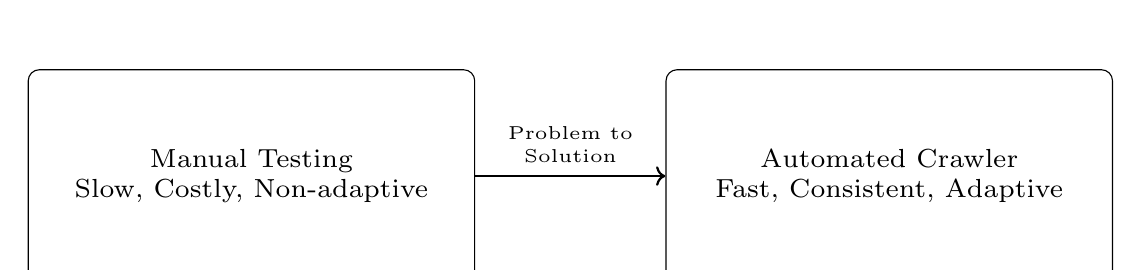
\begin{tikzpicture}[scale=1.35,every node/.style={align=center,transform shape,font=\scriptsize}]
  \node[draw, rounded corners, minimum width=4.2cm, minimum height=2cm] (manual) at (0,0) {Manual Testing\\Slow, Costly, Non-adaptive};
  \node[draw, rounded corners, minimum width=4.2cm, minimum height=2cm] (auto) at (6,0) {Automated Crawler\\Fast, Consistent, Adaptive};
  \draw[thick, ->] (manual) -- node[above, font=\tiny]{Problem to \\Solution} (auto);
\end{tikzpicture}
\caption{Transition from Manual to Automated Testing}
\label{fig:manual-to-auto}
\end{figure}

\section{Motivation}

We were motivated by the idea of making professional security testing tools available to everyone. Small businesses and developers often skip security audits because they are too expensive or complicated. Wibe Crawler aims to change this by providing a powerful but easy-to-use platform that handles the repetitive work of finding vulnerabilities.

\section{Objectives}

The primary objectives of the Wibe Crawler project are:

\begin{enumerate}
  \item \textbf{Desktop App:} Build a cross-platform desktop application using Electron, Svelte 5, and TailwindCSS.
  \item \textbf{Intelligent Crawler:} Create a Puppeteer-based crawler that can automatically handle forms, cookies, and site mapping.
  \item \textbf{AI Analysis:} Integrate the Groq AI engine to analyze security data with a system that manages multiple API keys to avoid limits.
  \item \textbf{Fuzzer:} Build a directory fuzzer to find hidden files and folders that scanners usually miss.
  \item \textbf{Reporting:} Automatically create PDF reports that explain vulnerabilities clearly and provide fixes.
  \item \textbf{Tool Orchestration:} Create a Backend Agent to run and coordinate external tools like nmap and sqlmap.
\end{enumerate}

\section{Scope and Deliverables}

The scope of the Wibe Crawler project is strictly defined to ensure technical feasibility, security, and focused research on AI-driven reconnaissance. The system is engineered to perform a non-destructive audit of web applications reachable via standard HTTP/HTTPS protocols.

\subsection{In-Scope Activities}
The project encompasses the following technical capabilities:
\begin{itemize}
    \item \textbf{Comprehensive Web Reconnaissance:} Implementation of a state-aware crawler using Puppeteer to navigate up to 1000 pages, extracting structural data including HTML forms, session cookies, and cross-domain links.
    \item \textbf{AI-Driven Vulnerability Orchestration:} Development of a parallel processing engine that clusters crawl data and utilizes Large Language Models (gpt-oss-120b) and specialized tools (nmap, sqlmap) to identify security anti-patterns.
    \item \textbf{Directory Fuzzing:} Integration of a concurrent HTTP probing module that uses customizable wordlists to discover hidden assets and directory structures often missed by standard crawlers.
    \item \textbf{Automated Security Reporting:} Generation of standardized PDF reports that include executive summaries, CVSS v3.1 severity scores, and verifiable HTTP request/response snippets.
\end{itemize}

\subsection{Out-of-Scope Constraints}
To maintain ethical standards and operational safety, the following activities are excluded from the current scope:
\begin{itemize}
    \item \textbf{Network-Layer Attacks:} Testing of non-web protocols (e.g., SSH, FTP, SMTP) or performing Denial-of-Service (DDoS) simulations.
    \item \textbf{Destructive Exploitation:} Automated execution of payloads that result in permanent data loss, server state changes, or account lockouts.
    \item \textbf{External API Auditing:} Deep analysis of third-party cloud services or APIs that are not directly hosted on the target domain.
\end{itemize}

\subsection{System Limitations}
The current implementation of Wibe Crawler is bounded by several technical and operational constraints documented during Phase 2 development:
\begin{itemize}
    \item \textbf{Inference Dependency:} Vulnerability detection accuracy is tied to the underlying Large Language Model's (gpt-oss-120b) reasoning capabilities; results are advisory and require human-in-the-loop validation.
    \item \textbf{Rate Limiting:} Performance may be throttled by the token quotas and latency of external AI inference APIs (e.g., Groq Cloud).
    \item \textbf{Protocol Focus:} The system operates exclusively at the Application Layer (Layer 7) and does not audit network-level or host-level infrastructure.
    \item \textbf{Anti-Bot Barriers:} Sophisticated anti-automation mechanisms like CAPTCHAs or behavioral fingerprinting currently limit the crawler's autonomous navigation on highly protected domains.
\end{itemize}

\subsection{Project Deliverables}
The project delivers a cohesive suite of artifacts, including:
\begin{itemize}
    \item \textbf{Software Artifacts:} A cross-platform Electron desktop application executable for Windows and Linux environments.
    \item \textbf{Technical Codebase:} Modular TypeScript source code for the Svelte 5 frontend, the specialized Node.js execution engines, and the Backend Agent service.
    \item \textbf{Security Documentation:} A comprehensive technical report detailing the project methodology, literature grounding, and phase-wise implementation progress.
    \item \textbf{Assurance Proofs:} Verifiable security finding logs and automated PDF reports generated from live system validation.
\end{itemize}

\section{Methodology Overview}
The development of Wibe Crawler follows a modular, three-layer architectural approach designed for high-performance automation and intelligent orchestration:
\begin{itemize}
    \item \textbf{Presentation Layer (Svelte 5):} Provides a reactive and intuitive user interface for scan configuration and real-time result visualization using Svelte Runes for optimal performance.
    \item \textbf{Orchestration Layer (Node.js/TypeScript):} Manages the concurrency of execution engines, handles data clustering for AI analysis, and coordinates the Backend Agent service via SSE (Server-Sent Events) to integrate external security tools.
    \item \textbf{Execution Layer (Puppeteer/Backend-Tools):} Performs state-aware crawling via a Native Crawler and orchestrates specialized security tools including nmap, sqlmap, nikto, and gobuster for multi-vector vulnerability discovery.
\end{itemize}
This methodology ensures that each component—from browser automation to specialized tool orchestration—operates with maximum efficiency and security, providing a robust foundation for autonomous penetration testing.

\section{Relevance to Industry and Society}
The development of Wibe Crawler addresses critical security gaps that extend beyond pure academic research, offering significant value to both the cybersecurity industry and the broader digital society:

\begin{itemize}
    \item \textbf{Democratizing Advanced Security:} By providing a high-performance, AI-augmented tool at a fraction of the cost of commercial enterprise suites, Wibe Crawler empowers Small and Medium-sized Enterprises (SMEs) to defend their digital assets. This contributes to a more equitable digital economy where robust security is accessible to all organizations, regardless of their scale or budget.
    \item \textbf{Closing the Discovery Gap:} In the era of Rapid Application Development and CI/CD, manual security testing is often the slowest link. Wibe Crawler provides the speed and consistency required to keep pace with modern deployment cycles, reducing the window of opportunity for malicious actors to exploit newly deployed vulnerabilities.
    \item \textbf{Protecting Public Data and Institutions:} As government and public institutions move services online, the security of their portals becomes a matter of public trust. Wibe Crawler assists in identifying vulnerabilities in institutional infrastructure, directly contributing to the protection of citizen data and the operational integrity of social and financial frameworks.
\end{itemize}
Ultimately, the project fosters a culture of proactive security, moving the industry toward a future where automated, intelligent reconnaissance is a standard pillar of digital resilience \cite{das2021, rehman2022}.

\section{Organization of the Report}

This report is structured to guide the reader through the lifecycle of the Wibe Crawler project, from its theoretical foundations to the final validated implementation. The content is organized into the following chapters:

\begin{enumerate}
    \item \textbf{Chapter 1: Introduction} establishes the foundational context of the project. It outlines the problem statement regarding existing manual penetration testing overheads, defines the primary objectives, and sets the technical scope, methodology overview, and broader socio-technical relevance of the research.
    \item \textbf{Chapter 2: Literature Review} provides an in-depth analysis of the current state of web security. It evaluates existing automated tools like Burp Suite and OWASP ZAP, and explores modern automation technologies such as Puppeteer and Playwright that form the technical basis of the crawler.
    \item \textbf{Chapter 3: Project Timeline} presents the project's developmental roadmap. It details the chronological milestones and task durations for the Phase 2 implementation via a technical Gantt Chart.
    \item \textbf{Chapter 4: System Requirements and Analysis} details the functional and non-functional requirements of the system. It provides a comprehensive specification of hardware and software needs and evaluates the project's viability through a multi-dimensional feasibility study.
    \item \textbf{Chapter 5: System Design} describes the high-level architecture and detailed design of the Wibe Crawler. It includes UML diagrams, algorithmic flowcharts, and the conceptual design of the user interface.
    \item \textbf{Chapter 6: Implementation} details the technical execution of the project. It covers the technology stack justification, implementation of key modules, and technical challenges overcome during development.
    \item \textbf{Chapter 7: Testing and Results} provides a comprehensive evaluation of the system. It outlines the testing methodology (functional testing, integration security validation, and pragmatic system-wide verification), presents a detailed execution summary and validation matrix, and analyzes the project's performance in real-world scenarios.
    \item \textbf{Chapter 8: Conclusions} synthesizes the research findings. It summarizes the project's technical accomplishments and reflects on its broader impact on the cybersecurity landscape and organizational resilience.
    \item \textbf{Chapter 9: Future Scope and Impact} looks beyond the current implementation. It discusses the technological roadmap for enhancement and explores the broader socio-technical impact (SDG 9 \& 16) and ethical considerations of the project.
    \item \textbf{Publications} (Post-Conclusions) documents the research outreach of the project. It includes the full citation for our accepted paper on RAG-driven penetration testing, the core abstract, and presentation certificates awarded to the team.
\end{enumerate}

The report also includes a comprehensive set of \textbf{Appendices} providing technical documentation, Dockerized installation guides, and core source code components essential for reproducing the system and understanding its underlying logic.
\chapter{Literature Review}
\label{chap:litreview}

\section{Existing Tools and Frameworks and Recent Research}

Several web security tools dominate the market, each providing a distinct approach to vulnerability detection. OWASP ZAP (Zed Attack Proxy) and sqlmap are integrated into the Wibe Crawler backend to automate database fingerprinting and injection testing \cite{zaproxy2024}. Similarly, Nikto and Nmap are utilized for comprehensive server-side misconfiguration analysis and port discovery. Burp Suite, particularly the Professional version, remains the industry standard for manual verification, while Wibe Crawler focuses on automating the "cognitive" analysis of these raw tool outputs via AI-driven classification. The OWASP Testing Guide (WSTG) serves as the definitive reference for these methodologies, providing a standardized framework for consistent and thorough security testing across all integrated modules \cite{owasp2024}.

Recent research further underscores the necessity of AI-driven approaches to handle the increasing complexity and asynchronous nature of modern web architectures. The transition to Svelte 5 and Tailwind CSS v4 in our implementation reflects the need for "zero-runtime" overhead in security dashboards as discussed by Liu et al. \cite{liu2025}. Wibe Crawler adopts priority-based logic by utilizing a native crawler that intercepts network traffic at the V8 engine level, providing deeper visibility than standard headless libraries. This is further supported by the work of Seker et al. (2025), whose research into AI agents demonstrates that multi-tool orchestration can significantly reduce false-positive rates \cite{seker2025}. 

The integration of Large Language Models (LLMs) like gpt-oss-120b via a Multi-Key Rotation Manager allows the system to sustain high-throughput analysis even under strict API rate limits. Roy et al. (2025) argued that by simulating adversarial reconnaissance patterns through AI, security tools can transition from reactive scanning to proactive risk modeling \cite{roy2025}. Our implementation of a Zod-based validation layer ensures that AI outputs are structurally sound, directly addressing the data integrity concerns raised by Das and Sandhane \cite{das2021}.

\section{Modern Web Automation Technologies}

Modern web automation frameworks are essential for effective security testing. During the research phase, several technologies were evaluated for Wibe Crawler's implementation:

\begin{itemize}
    \item \textbf{Puppeteer}: A high-level Node.js API provided by the Google Chrome team for Chromium automation. Unlike traditional Selenium, Puppeteer communicates directly with the browser via the DevTools Protocol, offering superior performance for tasks like form submission, cookie management, and PDF generation. Its native support for modern JavaScript features and Single Page Applications (SPAs) makes it the ideal candidate for a security-focused crawler~\cite{puppeteer2025}.
    \item \textbf{Selenium}: An industry-standard WebDriver that supports multiple browsers and languages. While highly versatile, its reliance on a middle-ware driver can introduce latency and complexity when handling modern, high-speed asynchronous interactions required for autonomous reconnaissance~\cite{selenium2025}.
    \item \textbf{Playwright}: A modern framework developed by Microsoft that builds upon the foundations of Puppeteer but adds cross-browser support (WebKit, Firefox) out of the box. While architecturally impressive, its broader scope was deemed redundant for Wibe Crawler, which leverages the standardized V8 engine found in Electron and Chromium for maximum stability~\cite{playwright2025}.
\end{itemize}

The effectiveness of these crawlers is a subject of ongoing study. Stafeev (2022) conducted an evaluation of crawling algorithms for web security measurements, identifying that "state-aware" crawling---where the crawler understands the current context of the application (e.g., logged-in vs. logged-out states)---is a key indicator of effectiveness~\cite{stafeev2022}. Wibe Crawler implements this by using a recursive state-validation function that checks specific login-indicators before every automated DOM interaction. Furthermore, the concept of site isolation and process separation within browsers, as discussed by Calzavara et al. (2021), is crucial for maintaining security during automated interactions, preventing cross-site leaks during the discovery process~\cite{calzavara}. We adopted this by leveraging Electron’s "Context Isolation," which creates a direct security boundary between our Puppeteer-driven browser engines and the system-level Node.js APIs. Rehman (2022) also noted the practical challenges in implementing AI for cybersecurity, particularly the high computational overhead and token-cost management, which Wibe Crawler aims to overcome through its modular "Orchestration Layer" and Groq-powered inference~\cite{rehman2022}. Our solution was to implement a "Structural Deduplication" module that prevents redundant AI analysis on pages with shared layouts, directly addressing the cost concerns raised in Rehman’s study.

After careful evaluation, Wibe Crawler was implemented using Puppeteer for its performance with modern web applications and seamless integration with Node.js and Electron. This choice, combined with Server-Sent Events (SSE) for low-latency communication between the Backend Agent and the user interface, provides the right balance of performance, reliability, and maintainability.

\section{Comparative Analysis of Security Tools}

To better understand the positioning of Wibe Crawler in the current security landscape, a comparative analysis was conducted against industry-standard tools. Table~\ref{tab:tool-comparison} summarizes the key differences in features, automation, and intelligence.

\begin{table}[ht]
\centering
\caption{Comparative Analysis of Web Security Tools}
\label{tab:tool-comparison}
\begin{tabularx}{\textwidth}{@{} l XXX @{}}
\toprule
\textbf{Feature} & OWASP ZAP & Burp Suite (Pro) & Wibe Crawler \\
\midrule
\textbf{Core Engine} & Java-based Proxy & Java-based Proxy & Node.js/Electron \\
\textbf{JS Rendering} & Limited (HtmlUnit) & Chromium Integration & native Puppeteer \\
\textbf{AI Analysis} & Manual / Plugins & Limited (Extensions) & Native Groq/gpt-oss-120b \\
\textbf{Orchestration} & Manual Configuration & Scanning Profiles & Backend Agent (nmap/sqlmap) \\
\textbf{Reporting} & Standard XML/HTML & Custom/Enterprise & Automated AI PDF \\
\textbf{Cost} & Open Source & Commercial License & Academic Project \\
\bottomrule
\end{tabularx}
\end{table}

\section{Comparative Analysis of Research Methodologies}

While Table~\ref{tab:tool-comparison} focuses on software features, Table~\ref{tab:research-comparison} evaluates Wibe Crawler against established academic frameworks for web reconnaissance and AI-driven security. This comparison highlights our implementation's alignment with contemporary research methodologies.

\begin{table}[ht]
\centering
\caption{Research methodology comparison}
\label{tab:research-comparison}
\begin{tabularx}{\textwidth}{@{} l XXX @{}}
\toprule
\textbf{Research Framework} & \textbf{Key Strategy} & \textbf{Wibe Crawler Implementation} \\
\midrule
Stafeev (2022) \cite{stafeev2022} & State-aware navigation & Login-context persistence via Puppeteer page objects. \\
Roy et al. (2025) \cite{roy2025} & Adversarial modeling & LLM-driven prioritization of high-value attack surfaces. \\
Seker et al. (2025) \cite{seker2025} & Multi-tool orchestration & Backend Agent layer integrating nmap, sqlmap, and nikto. \\
Rehman (2022) \cite{rehman2022} & Computational efficiency & Structural deduplication to reduce AI inference costs. \\
\bottomrule
\end{tabularx}
\end{table}

\section{Gap Analysis}
\label{sec:gapanalysis}

The current security testing landscape, while robust in many aspects, reveals several critical gaps that Wibe Crawler is specifically designed to address. This analysis informs the "Autonomous Reconnaissance" philosophy of the project.

\subsection{Intelligence vs. Scripted Automation Gap}
Most existing tools focus on \textit{automation}---the repetition of predefined sequences---rather than \textit{intelligence}---the ability to adapt to new, unforeseen data structures. Traditional scanners often fail when encountering non-standard navigation patterns, custom API schemas, or complex multi-step workflows. Wibe Crawler bridges this gap by integrating an LLM-based reasoning engine (gpt-oss-120b). Instead of simply "following links," the system performs semantic analysis of the Document Object Model (DOM), allowing it to prioritize high-risk areas like administrator panels or sensitive debug endpoints based on their functional purpose rather than just their URL structure.

\subsection{Modern Web Architecture \& Shadow DOM Adaptability Gap}
Traditional scanners often struggle with the "Headless-Hydration" problem prevalent in modern React, Svelte, and Vue applications. These apps often appear as empty shells to traditional HTTP-client-based crawlers that lack V8 engine execution. Furthermore, the increasing use of the \textit{Shadow DOM} creates encapsulation boundaries that many tools cannot penetrate. By utilizing headless Chromium via Puppeteer at its core, Wibe Crawler ensures that the application is fully "hydrated" and rendered before analysis begins. This ensures that components like dynamically generated modals, custom web components, and shadow-root elements are included in the security audit.

\subsection{State-Aware Dynamic Interaction Gap}
Advanced vulnerabilities often reside behind specific application states (e.g., being logged in as a specific role or having a particular session flag set). Existing tools often lose context during deep-crawling, leading to "log-out loops" or broken session states. Wibe Crawler implements a \textit{State-Aware Execution Layer} that monitors cookies, LocalStorage, and JWT headers in real-time. This allows the system to maintain its authorization context even when performing destructive fuzzing or navigating complex single-page application (SPA) state transitions.

\subsection{The "Black-Box" Transparency \& Verification Gap}
A major pain point in enterprise security is the "Evidence Gap," where tools provide findings without the raw technical proof required for remediation. This leads to user skepticism and slower fix cycles. Wibe Crawler addresses this by serving as a transparent proxy during its analysis phase, capturing and providing raw HTTP request/response snippets for every detected vulnerability. This transparency ensures that its AI-driven findings are immediately verifiable by human security analysts, fostering a collaborative security workflow rather than just a list of alerts.

\subsection{Resource Accessibility \& Operational Complexity Gap}
The complexity of configuring enterprise-grade tools like Burp Suite Enterprise or Tenable often necessitates a specialized security team, which many organizations lack. This creates a "Security Debt" for small-to-medium enterprises (SMEs). Wibe Crawler simplifies this through a unified "Project-Based" GUI built on Svelte 5. By abstracting the complexity of fuzzer wordlists and AI prompt engineering into intuitive "One-Click" workflows, it makes advanced reconnaissance and vulnerability assessment accessible to DevOps engineers and software developers.

\subsection{Key Differentiators}

\begin{itemize}
  \item \textbf{Autonomous Orchestration:} LLM-driven decision making that adapts to target application logic.
  \item \textbf{V8 Native Execution:} Superior handling of SPA hydration, JavaScript execution, and web components.
  \item \textbf{Evidence-Based Reporting:} Direct linking of vulnerability findings to raw HTTP evidence.
  \item \textbf{High-Speed Inference:} Leverages Groq Cloud for near-instant AI analysis during the crawling phase.
  \item \textbf{Modular Elasticity:} Decoupled execution engines (Crawler/Fuzzer) integrated through a unified agent layer.
\end{itemize}

By addressing these critical gaps, Wibe Crawler represents a significant advancement in web security testing tools, transforming the scanning process from a manual, configuration-heavy task into an intelligent, autonomous operation.

\chapter{Project Timeline}
\label{chap:timeline}

\section{Gantt Chart}

\begin{figure}[ht]
\centering
\includegraphics[width=\textwidth]{gantt.png}
\caption{Gantt Chart for Project Phase 2}
\label{fig:gantt-phase2}
\end{figure}

The Phase 2 development lifecycle follows a structured 10-week timeline (as illustrated in Figure~\ref{fig:gantt-phase2}), transitioning from architectural foundation to advanced AI-driven security orchestration. The implementation schedule is organized as follows:

\begin{itemize}
  \item \textbf{Weeks 1--2: Foundation Integration and Desktop Scaffolding} --- This initial phase focused on porting the core scouting logic from Phase 1 into a robust \textbf{Electron} desktop environment. Key activities included establishing the secure \textbf{Inter-Process Communication (IPC)} bridge, configuring the build system for \textbf{Svelte 5}, and ensuring that the Node.js main process could reliably spawn headless browser instances without memory overhead.
  
  \item \textbf{Weeks 3--4: Reactive UI and Telemetry Design} --- Development focused on the "Presentation Layer." We implemented a \textbf{Glassmorphic Dashboard} using Svelte 5 and Tailwind CSS, prioritizing real-time responsiveness via \textbf{Server-Sent Events (SSE)}. This involved setting up a centralized state management system to handle live telemetry data from active scans.
  
  \item \textbf{Weeks 5--6: Advanced Crawler and State Management} --- The execution engine was upgraded from simple link-following to a \textbf{State-Aware Puppeteer Crawler}. This involved implementing logic to handle Single-Page Application (SPA) hydration, capturing session cookies and JWTs for authenticated crawling, and developing an automated form-detection module.
  
  \item \textbf{Weeks 7--8: AI Orchestration and Parallel Processing} --- This was the core "Intelligence" phase. We implemented the \textbf{Queue-Based Worker Pool} for managing Groq API keys. The system was designed to perform "Data Clustering," where large crawl datasets are split into manageable chunks and analyzed in parallel by \textbf{gpt-oss-120b}. This phase also included refining the prompt engineering to ensure consistent CVSS v3.1 scoring and CWE classification.
  
  \item \textbf{Week 9: Fuzzer Integration and Automated Reporting} --- We integrated the high-concurrency \textbf{Directory Fuzzer}. Concurrently, the client-side \textbf{jsPDF Reporting Engine} was implemented, allowing users to transform AI findings into professional, verifiable security reports with one-click functionality.
  
  \item \textbf{Week 10: Optimization, Review, and Finalization} --- The final week was dedicated to system-wide \textbf{Performance Optimization} and the integration of a \textbf{Backend Agent} service for external tool orchestration. This included benchmarking the fuzzer's thread efficiency, stress-testing the AI analyzer with high-volume datasets, and final documentation synthesis. The phase concluded with a comprehensive functional review to ensure the system met all Phase 2 deliverables.
\end{itemize}

\chapter{System Requirements and Analysis}
\label{chap:requirements}

\section{Introduction to Requirement Analysis}
Requirement analysis is a fundamental process in the software development lifecycle that involves defining, documenting, and maintaining the requirements for the Wibe Crawler project. This process ensures that the system meets the technical and operational needs of cybersecurity professionals while maintaining ethical and functional boundaries. By identifying the specific needs of the users and the technical environment, this analysis provides a clear roadmap for the implementation of the three-layer architecture.

\section{Functional Requirements (FRs)}
Functional requirements define the specific features and behaviors that the Wibe Crawler must possess to achieve its objectives:
\begin{itemize}
    \item \textbf{FR1: Recursive Web Crawling:} The system must be capable of navigating target domains recursively, extracting navigable links, and handling Single-Page Application (SPA) hydration.
    \item \textbf{FR2: Parallel Directory Fuzzing:} The system must support concurrent directory discovery using customizable wordlists to identify unlinked assets and hidden endpoints.
    \item \textbf{FR3: AI-Driven Vulnerability Identification:} The system must integrate a Large Language Model (gpt-oss-120b) to analyze gathered data and identify security anti-patterns aligned with the OWASP Top 10.
    \item \textbf{FR4: Automated PDF Reporting:} The system must provide a one-click mechanism to generate professional security reports containing vulnerability details and technical evidence.
    \item \textbf{FR5: Target Environment Management:} The system must allow users to configure scan targets, including protocol selection (HTTP/HTTPS) and session authentication context.
    \item \textbf{FR6: Multi-tool Security Orchestration:} The system must be capable of orchestrating external security tools (nmap, sqlmap, nikto) via a Backend Agent service to perform cross-layer vulnerability discovery.
\end{itemize}

\section{Non-Functional Requirements (NFRs)}
Non-functional requirements specify the criteria used to judge the operation of the system rather than specific behaviors:
\begin{itemize}
    \item \textbf{Performance:} The system must process crawling and fuzzing tasks with high concurrency without causing significant latency in the user interface.
    \item \textbf{Scalability:} The architecture must support the analysis of large-scale web applications with up to 1000 navigable pages.
    \item \textbf{Security:} The system must maintain isolation between crawling engines and the main application process to prevent client-side exploits from affecting the host machine.
    \item \textbf{Usability:} The dashboard must provide a responsive and intuitive experience, allowing users of varying technical skills to initiate and monitor scans easily.
    \item \textbf{Reliability:} The crawler must handle network timeouts and server-side rate limits gracefully through adaptive retry mechanisms.
\end{itemize}

\section{System Requirements Specification (SRS)}
This section details the hardware and software components required to deploy and operate the Wibe Crawler application.

\subsection{Hardware Requirements}
For the optimal operation of the Wibe Crawler desktop application, particularly during high-concurrency scans and AI orchestration, the following hardware specifications are recommended:
\begin{itemize}
    \item \textbf{Processor:} Intel Core i5 or AMD Ryzen 5 (Equivalent or higher) for multi-threaded processing.
    \item \textbf{Memory (RAM):} Minimum 8GB (16GB recommended) to accommodate multiple headless browser instances and the Node.js main process.
    \item \textbf{Storage:} 500MB of available space for application installation and scan report storage.
    \item \textbf{Network:} Stable broadband connection (100 Mbps recommended) for effective remote target reconnaissance.
\end{itemize}

\subsection{Software Requirements}
The Wibe Crawler is built upon a modern specialized software stack to ensure cross-platform compatibility and high-performance execution:
\begin{itemize}
    \item \textbf{Operating System:} Windows 10/11, Ubuntu 20.04+, or macOS Catalina+ (64-bit).
    \item \textbf{Build Tooling:} Bun (v1.2+) or Node.js (v22+) with Vite (v7+).
    \item \textbf{Frontend Stack:} Svelte 5 (Runes) with Tailwind CSS v4 "Zero-runtime" styling.
    \item \textbf{Core Engines:} Electron (v37+), Puppeteer (v24+), and Backend Agent Service.
    \item \textbf{Infrastructure:} Docker (v27+) for containerized tool orchestration and environment isolation.
    \item \textbf{AI \& APIs:} Groq Cloud API (gpt-oss-120b) and jsPDF for client-side reporting.
\end{itemize}

\section{Feasibility Study}
A feasibility study was conducted to evaluate the technical, operational, and economic viability of the project.

\subsection{Technical Feasibility}
The project leverages mature and battle-tested technologies like Electron and Puppeteer, while integrating cutting-edge AI via the Groq LPU architecture. The modular architecture ensures that complex task like browser automation and LLM inference can be handled without architectural bottlenecks. The availability of high-speed AI inference via Groq confirms that real-time security analysis is technically achievable within the current hardware ecosystem.

\subsection{Operational Feasibility}
The system is designed with an intuitive GUI that abstracts the complexity of terminal-based security tools. This ensures that the application can be operated by security analysts and developers with minimal training. The automated nature of the "Discover-Analyze-Report" loop significantly reduces the human effort required for comprehensive web reconnaissance, making the system highly feasible for integration into standard security workflows.

\subsection{Economic Feasibility}
By utilizing open-source frameworks (Electron, Svelte 5) and leveraging flexible AI API models (Groq), the project minimizes development and operational costs. For organizations, Wibe Crawler provides a low-cost alternative to expensive enterprise security suites, delivering high-end AI discovery capabilities with minimal infrastructure overhead. This makes the project economically viable for academic purposes and future industry adoption.

\chapter{System Design}
\label{chap:systemdesign}

\section{Architectural Design}
\label{sec:architecturaldesign}

Wibe Crawler is built upon a sophisticated three-layer architecture designed for high-performance autonomous security testing. This decoupling ensures that computationally intensive AI analysis and browser automation do NOT interfere with the responsiveness of the user interface.

\begin{enumerate}
  \item \textbf{Presentation Layer (Frontend):} Developed using \textbf{Svelte 5}, this layer provides a high-performance reactive dashboard. It utilizes \textbf{Runes} for optimal DOM reactivity and real-time visualization of scanner telemetry.
  
  \item \textbf{Orchestration Layer (The "Brain"):} This layer implements a \textbf{Multi-Key Rotation Manager} to handle high-throughput Groq AI analysis. It orchestrates the \textbf{Backend Agent Service}, which manages specialized tools via Server-Sent Events (SSE).
  
  \item \textbf{Execution Layer (The "Engines"):} 
  \begin{itemize}
    \item \textbf{Native Crawler:} A specialized engine using Electron's \textbf{BrowserWindow} for stealthy, high-visibility reconnaissance.
    \item \textbf{Backend Tools:} Specialized security engines including \textbf{nmap, sqlmap, nikto, and gobuster} for deep infrastructure analysis.
  \end{itemize}
\end{enumerate}

\subsection{Electron Process Model}

The system leverages Electron's multi-process architecture to ensure security and performance stability:

\begin{itemize}
  \item \textbf{Main Process (Host Environment):} Operating in a full Node.js environment, the Main Process serves as the "System Orchestrator." It manages the \textbf{Native Crawler} threads, coordinates with the \textbf{SSE Backend}, and handles the KeyManager for AI analysis.
  
  \item \textbf{Renderer Process (UI Environment):} Responsible for the Svelte 5 dashboard. It operates in a sandboxed environment, managing the \textbf{jsPDF-based report generation} and visualizing scan results.
\end{itemize}

To formalize the interaction between the user and the automated scanning engines, a Use Case Diagram was developed (Figure~\ref{fig:use-case}). This diagram establishes the primary operational boundaries and the system’s response handling during a security audit.

\begin{figure}[ht]
\centering
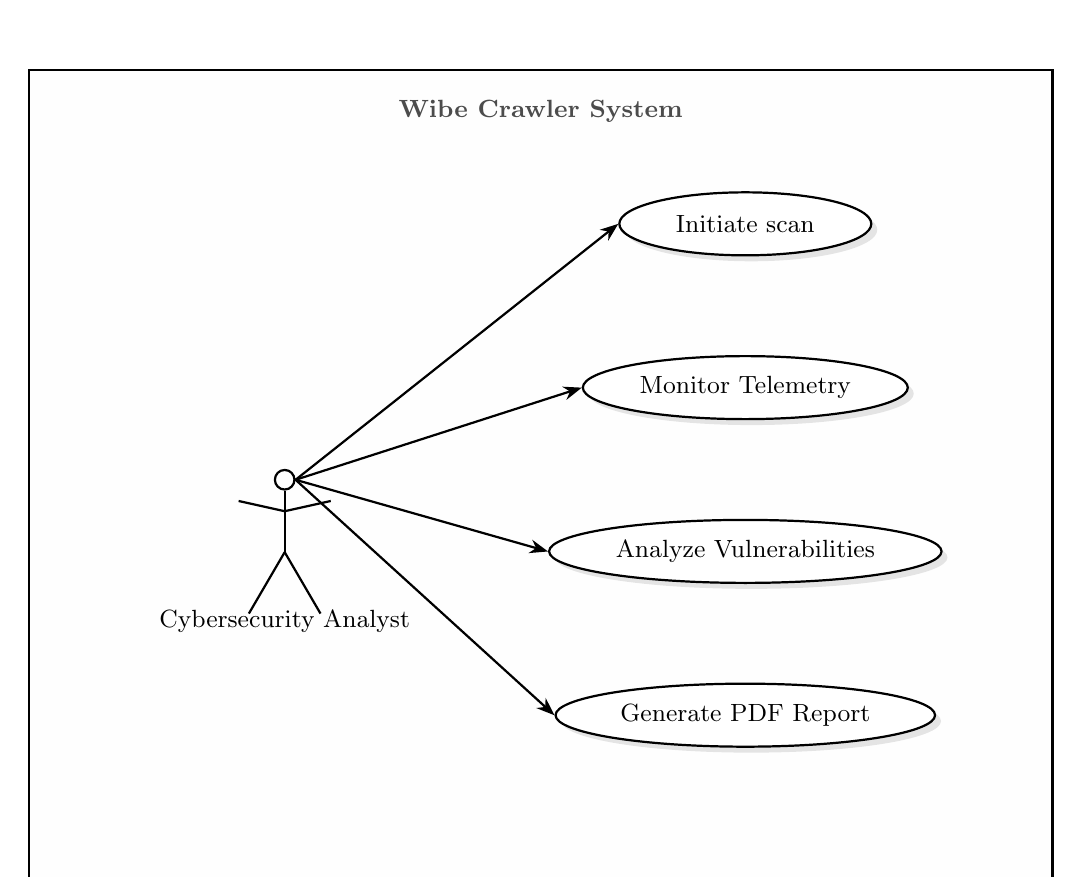
\begin{tikzpicture}[
    scale=1.3, 
    every node/.style={font=\small},
    usecase/.style={draw, ellipse, minimum width=3.2cm, minimum height=0.8cm, thick, fill=white, drop shadow={opacity=0.2}, align=center}
]
% Boundary (Refined styling)
\fill[lightgrey!10] (-2.5,-6.5) rectangle (7.5,1.5);
\draw[thick] (-2.5,-6.5) rectangle (7.5,1.5);
\node[anchor=north, font=\bfseries\small, text=darkgrey] at (2.5,1.3) {Wibe Crawler System};

% Actor (Refined stick figure)
\node (analyst) [draw, circle, inner sep=2.5pt, thick, label={[label distance=1.4cm]below:Cybersecurity Analyst}] at (0,-2.5) {};
\draw [thick] (analyst.south) -- ++(0,-0.6) coordinate (torso);
\draw [thick] (torso) -- ++(-0.35,-0.6);
\draw [thick] (torso) -- ++(0.35,-0.6);
\draw [thick] (torso)++(0,0.4) -- ++(-0.45,0.1);
\draw [thick] (torso)++(0,0.4) -- ++(0.45,0.1);

% Use Cases (With improved styles)
\node (uc1) [usecase] at (4.5,0) {Initiate scan};
\node (uc2) [usecase] at (4.5,-1.6) {Monitor Telemetry};
\node (uc3) [usecase] at (4.5,-3.2) {Analyze Vulnerabilities};
\node (uc4) [usecase] at (4.5,-4.8) {Generate PDF Report};

% Relationships
\draw [->, >=Stealth, thick] (analyst.east) -- (uc1.west);
\draw [->, >=Stealth, thick] (analyst.east) -- (uc2.west);
\draw [->, >=Stealth, thick] (analyst.east) -- (uc3.west);
\draw [->, >=Stealth, thick] (analyst.east) -- (uc4.west);
\end{tikzpicture}
\caption{System Use Case Diagram}
\label{fig:use-case}
\end{figure}

\section{Algorithmic Design}

The system's core logic is governed by a state-aware synchronization algorithm that coordinates the parallel execution of the crawling and fuzzing engines. This process ensures that data gathered from the network layer (fuzzing) and application layer (crawling) is merged seamlessly before AI analysis.

\subsection{System Operational Flowchart}

\begin{figure}[H]
\centering
\resizebox{0.98\textwidth}{!}{%
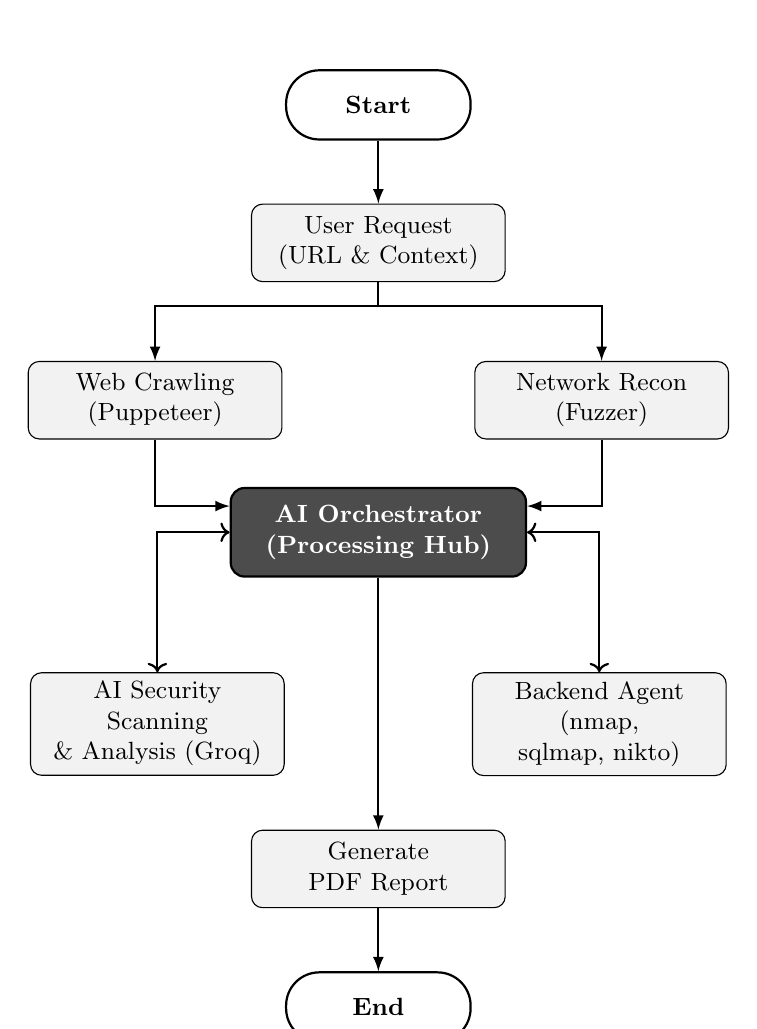
\begin{tikzpicture}[
    node distance=0.8cm and 1.2cm,
    auto,
    block/.style={rectangle, draw, rounded corners, text width=8.5em, text centered, minimum height=2.8em, fill=lightgrey, font=\small},
    hub/.style={rectangle, draw, rounded corners=0.5em, text width=10em, text centered, minimum height=3.2em, fill=darkgrey, text=white, font=\small\bfseries, thick},
    terminal/.style={rectangle, draw, rounded corners=1.2em, text width=6em, text centered, minimum height=2.5em, fill=white, font=\small\bfseries, thick},
    line/.style={draw, thick, -latex}
  ]
    % Nodes - Sequential Execution Flow
    \node [terminal] (start) {Start};
    \node [block, below=of start] (request) {User Request\\(URL \& Context)};
    
    % Phase 1: Reconnaissance (Parallel)
    \node [block, below left=1.0cm and -0.4cm of request] (crawl) {Web Crawling\\(Puppeteer)};
    \node [block, below right=1.0cm and -0.4cm of request] (fuzz) {Network Recon\\(Fuzzer)};
    
    % Phase 2: AI Orchestrated Analysis
    \node [hub, below=2.6cm of request] (agent) {AI Orchestrator\\(Processing Hub)};
    \node [block, below left=1.2cm and -0.7cm of agent] (scan) {AI Security Scanning\\\& Analysis (Groq)};
    \node [block, below right=1.2cm and -0.7cm of agent] (backend) {Backend Agent\\(nmap, sqlmap, nikto)};
    
    % Phase 3: Final Output
    \node [block, below=3.2cm of agent] (pdf) {Generate PDF Report};
    \node [terminal, below=of pdf] (end) {End};

    % Phase 1 Paths
    \path [line] (start) -- (request);
    \path [line] (request.south) -- ++(0,-0.3) -| (crawl.north);
    \path [line] (request.south) -- ++(0,-0.3) -| (fuzz.north);
    
    % Phase 2 Paths (Input to Orchestrator - Non-overlapping)
    \path [line] (crawl.south) |- (agent.170);
    \path [line] (fuzz.south) |- (agent.10);
    
    % Analysis and Report (Bidirectional + Central Flow)
    \path [line] (agent.south) -- (pdf.north);
    \path [line, <->] (agent.west) -| (scan.north);
    \path [line, <->] (agent.east) -| (backend.north);
    \path [line] (pdf) -- (end);
    
\end{tikzpicture}
}
\caption{System Operational Flowchart}
\label{fig:system-flowchart}
\end{figure}

The \textbf{System Operational Flowchart} (Figure~\ref{fig:system-flowchart}) illustrates the end-to-end lifecycle of a security audit within Wibe Crawler. This autonomous process is structured into five core functional phases:

\begin{enumerate}
    \item \textbf{Phase 1: Session Initialization} --- The process begins with the \textbf{User Request}, where the target URL is provided along with optional session context (e.g., authentication headers or cookies). This stage ensures the crawler’s environment is correctly configured for the specific target application.
    
    \item \textbf{Phase 2: Parallel Autonomous Discovery} --- Upon initialization, the system spawns two concurrent discovery engines. The \textbf{Web Crawling engine} (Puppeteer) performs deep recursive DOM analysis and link extraction, while the \textbf{Network Recon engine} (Fuzzer) identifies unlinked assets and hidden directory structures.
    
    \item \textbf{Phase 3: The AI Orchestrator (Central Processing Hub)} --- Raw data from both discovery engines is funneled into the \textbf{AI Orchestrator}. This central "Processing Hub" implements a \textbf{Multi-Key Rotation Manager} to sustain high-throughput operation. It performs data normalization and aggregates findings into "Contextual Clusters" ready for deeper analysis.
    
    \item \textbf{Phase 4: Coordinated Security Analysis} --- The Processing Hub coordinates two specialized analysis layers. The \textbf{Groq AI Layer} (gpt-oss-120b) perform semantic vulnerability classification, while the \textbf{Backend Agent} orchestrates industrial tools like \textbf{nmap, sqlmap, and nikto} for technical validation. This bidirectional flow ensures that findings are cross-verified before reporting.
    
    \item \textbf{Phase 5: Automated Reporting and Closure} --- The final phase involves the \textbf{Generation of the PDF Report}. The validated findings are synthesized into a professional document using the \textbf{jsPDF} engine, providing executive summaries and prioritized remediation steps.
\end{enumerate}

\section{Threat Model}

To provide a focused security analysis, the development of Wibe Crawler is guided by a specific threat model. Defining this model ensures that the system's vulnerability detection logic is optimized for the most relevant attack vectors while maintaining clear operational boundaries.

\subsection{Attacker Model}
The system assumes an \textbf{External Unauthenticated Attacker}. This is a threat actor who does not possess valid credentials but attempts to discover weaknesses in the application's public attack surface through reconnaissance and fuzzing.

\subsection{Risk Assumptions and Scope Boundaries}
The operational scope of Wibe Crawler is strictly limited to the \textbf{Application Layer (Web Layer)}. The following boundaries and assumptions define the system's security focus:

\begin{itemize}
  \item \textbf{Web-Layer Focus:} The system primarily analyzes HTTP/HTTPS traffic, DOM structures, and client-side interactions.
  \item \textbf{Infrastructure Reconnaissance:} Utilizing the \textbf{Backend Agent (nmap)}, the system performs non-destructive port discovery and service fingerprinting to identify potential entry points for web-layer attacks.
  \item \textbf{No Destructive Network Attacks:} The system does not perform ARP spoofing, DHCP starvation, or other destructive network-layer exploits.
  \item \textbf{No Internal Privilege Escalation:} The tool identifies vulnerabilities within the application (e.g., IDOR, Injection); it does not attempt host-based privilege escalation.
\end{itemize}

\section{User Interface (UI) Design}

The following screenshots (Figures~\ref{fig:ss-urls-design} through \ref{fig:ss-pdf-remediation-design}) illustrate the developed interface of the Wibe Crawler desktop application, showcasing the integration of high-speed reconnaissance and AI-driven analysis.

\clearpage
\begin{figure}[H]
\centering
\rotatebox{90}{
\begin{minipage}{0.9\textheight}
\centering
\includegraphics[width=\linewidth]{ss1.png}
\caption{Reconnaissance Dashboard showing crawled pages}
\label{fig:ss-urls-design}
\end{minipage}
}
\end{figure}

\clearpage
\begin{figure}[H]
\centering
\rotatebox{90}{
\begin{minipage}{0.9\textheight}
\centering
\includegraphics[width=\linewidth]{ss2.png}
\caption{AI-identified vulnerabilities with severity classification}
\label{fig:ss-vulnerabilities-design}
\end{minipage}
}
\end{figure}

\clearpage
\begin{figure}[H]
\centering
\rotatebox{90}{
\begin{minipage}{0.9\textheight}
\centering
\includegraphics[width=\linewidth]{ss3.png}
\caption{Generated PDF report: Executive Summary}
\label{fig:ss-pdf-summary-design}
\end{minipage}
}
\end{figure}


\clearpage
\begin{figure}[H]
\centering
\rotatebox{90}{
\begin{minipage}{0.9\textheight}
\centering
\includegraphics[width=\linewidth]{ss4.png}
\caption{Generated PDF report: Detailed Findings}
\label{fig:ss-pdf-findings-design}
\end{minipage}
}
\end{figure}

\clearpage
\begin{figure}[H]
\centering
\rotatebox{90}{
\begin{minipage}{0.9\textheight}
\centering
\includegraphics[width=\linewidth]{ss5.png}
\caption{Generated PDF report: Prioritized Remediation Recommendations}
\label{fig:ss-pdf-remediation-design}
\end{minipage}
}
\end{figure}

\chapter{Implementation}
\label{chap:implementation}

\section{Technology Stack Justification}

The selection of the technology stack for Wibe Crawler was not merely based on popularity, but on specific technical requirements for building a performant, autonomous security testing suite:

\begin{itemize}
    \item \textbf{Electron (Framework):} Traditional web-based security tools often struggle with the "Same-Origin Policy" and restricted filesystem access. Electron was chosen because it allows the system to operate in a \textbf{Native OS Environment} \cite{electron2025}. This enables the crawler to navigate between different domains without sandbox restrictions and permits direct disk access for storing detailed scan logs and generating structured PDF reports locally. its multi-process model further ensures that a crash in the browser automation layer does not affect the main application state.
    
    \item \textbf{Puppeteer (Crawl Engine):} To perform high-fidelity web crawling, we integrated \textbf{Puppeteer}, a Node.js library which provides a high-level API to control headless Chrome \cite{puppeteer2025}. This allows Wibe Crawler to execute JavaScript, handle single-page applications (SPAs), and extract forensic data from the DOM with the precision of a real browser. Unlike simple HTTP request-based crawlers, Puppeteer enables the discovery of assets that are only revealed after client-side rendering.
    
    \item \textbf{Svelte 5 (User Interface):} In a security scanner, the dashboard must visualize a high volume of real-time data. Unlike React, which uses a Virtual DOM, Svelte 5 utilizes \textbf{Runes} for fine-grained reactivity \cite{svelte2025}. This approach ensures that updates to the UI occur only where data has changed, resulting in a nearly instantaneous responsiveness with zero-runtime overhead. This is critical for maintaining fluid visualization while receiving high-throughput SSE streams from the backend.
    
    \item \textbf{Groq Cloud Inference (AI Engine):} Autonomous vulnerability analysis requires reasoning capabilities that only large models like \textbf{gpt-oss-120b} can provide \cite{gptoss2025}. However, LLM inference is traditionally slow. Groq's \textbf{Language Processing Unit (LPU)} architecture was selected for its revolutionary inference speeds \cite{groq2025}. This allows Wibe Crawler to perform deep semantic analysis on complex clusters in milliseconds. The implementation includes a \textbf{Multi-Key Rotation Manager} to sustain high-throughput scans without API quota interruptions.
    
    \item \textbf{Backend Agent Orchestration (Node.js):} To bridge the gap between web crawling and industrial security tools, we implemented a specialized \textbf{Backend Agent}. This service orchestrates \textbf{nmap, sqlmap, and nikto} asynchronously, streaming real-time security events back to the Svelte 5 dashboard via \textbf{Server-Sent Events (SSE)}. This ensures a unified, low-latency telemetry experience for the user.

    \item \textbf{Docker (Containerization):} A key challenge in security testing is the "Dependency Hell" associated with various security tools. We utilized \textbf{Docker} to containerize the Backend Agent and its dependencies \cite{docker2025}. This ensures that tools like \texttt{sqlmap} and \texttt{nmap} run in a consistent, isolated environment regardless of the host OS, preventing version conflicts and enhancing the overall security of the testing infrastructure.
    
\end{itemize}

\section{Challenges Faced During Implementation}

The development of Wibe Crawler presented several technical challenges that required innovative solutions (summarized in Table~\ref{tab:challenges}) to ensure optimal performance and reliability.

\begin{itemize}
  \item \textbf{AI Rate Limiting:} Solved via a \textbf{Multi-Key Rotation Manager} that monitors API quotas and automatically switches keys on cooldown.
  \item \textbf{AI Output Reliability:} Addressed using \textbf{Zod-based schema validation} to ensure AI responses are structurally sound for report generation.
  \item \textbf{Payload Constraints:} Optimized via \textbf{Semantic Data Clustering}, grouping crawl results into manageable batches for the LLM.
\end{itemize}

\begin{table}[ht]
\centering
\caption{Challenges and Mitigation Strategies}
\label{tab:challenges}
\begin{tabular}{|l|p{6cm}|}
\hline
\textbf{Challenge} & \textbf{Solution} \\
\hline
AI Rate Limiting & Multi-key rotation with automatic cooldown handling \\
\hline
AI Data Integrity & Zod-based validation and recursive extraction strategies \\
\hline
Large Payload & Semantic clustering and intelligent asset sampling \\
\hline
Form Interaction & Native browser context injection and stealthy re-play \\
\hline
\end{tabular}
\end{table}




\section{Implementation Details of Key Modules}

The project was executed using an \textbf{Agile-Scrum} inspired methodology, optimized for high-intensity research and rapid prototyping. This approach facilitated iterative development, allowing technical challenges encountered in the Execution layer to inform design adjustments in the Orchestration layer.

\subsection{Iterative Development Workflow}
Development was structured into two-week "Sprints," each focusing on a specific functional module. Frequent code reviews and system validation tests ensured that the integration of diverse technologies—Electron, Svelte 5, Puppeteer, and Groq—remained cohesive. The use of \textbf{Git} for version control allowed for decoupled development of the frontend and backend engines, enabling parallel work on the UI and the security scanning logic.

\subsection{Phase I: Foundations and Reconnaissance Infrastructure}
The initial phase was dedicated to building the "Physical" scanning layer.
\begin{itemize}
  \item \textbf{Core Browser Bridge:} Implementation of the initial Puppeteer execution engine, focusing on reliable DOM navigation and synchronous element detection.
  \item \textbf{Electron Shell Scaffolding:} Development of the multi-process architecture and secure IPC communication channels utilizing Context Isolation and the Context Bridge.
  \item \textbf{Reactive Dashboard Foundation:} Design of the primary Svelte 5 UI components and global state management system (Svelte Store) for handling real-time telemetry.
\end{itemize}

\subsection{Phase II: AI Orchestration and Intelligence Integration}
The second phase focused on the "Cognitive" analysis layer.
\begin{itemize}
  \item \textbf{AI Orchestration Engine:} Integration of the Groq Cloud API and development of the \textbf{Queue-Based Worker Pool} for handling concurrent API requests and LPU-powered inference.
  \item \textbf{Advanced Security Logic:} Implementation of the \textbf{Data Clustering} algorithms and prompt refinement for gpt-oss-120b to achieve accurate vulnerability classification and remediation mapping.
  \item \textbf{Autonomous Reporting Module:} Development of the client-side PDF generation engine using \textbf{jsPDF}, enabling the transformation of raw AI findings into professional, verifiable security reports.
\end{itemize}

\section{Technical Deep Dive of Core Modules}

To appreciate the system's operational complexity, it is necessary to examine the technical implementation of its three primary orchestration subsystems.

\subsection{Backend Agent Service Orchestration}
The \textbf{Backend Agent} is a decoupled Node.js service that acts as a bridge between the Electron frontend and industrial-grade CLI security tools. This module utilizes the \textbf{Child Process} API to spawn asynchronous instances of \textbf{Nmap, Sqlmap, and Nikto}. 
\begin{itemize}
    \item \textbf{Asynchronous Execution:} Tools are executed in separate threads to prevent blocking the main event loop, ensuring that the crawler remains responsive during intensive network scans.
    \item \textbf{Event-Driven Telemetry:} The agent parses the raw stdout of these tools in real-time. Instead of waiting for a tool to finish, it emits intermediate "Security Events" via a persistent \textbf{Server-Sent Events (SSE)} stream. This allows the dashboard to visualize "ports discovered" or "vulnerabilities identified" the moment they occur.
\end{itemize}

\subsection{AI Data Pipeline \& Clustering Logic}
The volume of raw data generated during a recursive crawl (HTML DOM, network headers, script sources) often exceeds the context window of modern LLMs. Wibe Crawler implements a \textbf{Semantic Data Pipeline} to mitigate this:
\begin{enumerate}
    \item \textbf{Forensic Extraction:} The system extracts security-relevant features such as form inputs, API endpoints, and JavaScript handlers.
    \item \textbf{Contextual Clustering:} These features are grouped into "Contextual Clusters" based on their functional similarity (e.g., all authentication-related forms are clustered together). 
    \item \textbf{Groq LPU Inference:} Clusters are sent to the \textbf{Groq LPU} in parallel batches. The AI performs semantic reasoning to identify vulnerabilities across the cluster, which is significantly more token-efficient than analyzing pages in isolation.
\end{enumerate}

\subsection{Secure Multi-Process Communication (IPC)}
In Wibe Crawler's architecture, the security of the application itself is paramount. We utilize a strict \textbf{Multi-Process Model} via Electron:
\begin{itemize}
    \item \textbf{Context Isolation:} The renderer process (Svelte 5 UI) has zero direct access to Node.js or the local filesystem. All dangerous operations are mediated by the main process.
    \item \textbf{The Context Bridge:} A secure \textbf{IPC Bridge} is established to handle telemetry. When a crawl engine discovers a link, it sends an IPC event to the Main process, which then broadcast the update to the UI. This ensures that even if a target website attempts a Cross-Site Scripting (XSS) attack against the scanner's dashboard, it cannot escape the browser sandbox to compromise the host system.
\end{itemize}

\chapter{Testing and Results}
\label{chap:testing}

\section{Introduction to Testing}

The testing phase is a critical component of the Wibe Crawler development lifecycle, ensuring that the integrated AI engines, crawling mechanisms, and user interface operate as a cohesive and reliable system. Testing was conducted iteratively to identify technical bottlenecks, validate security logic correctness, and ensure that the application handles edge cases—such as network latencies and malformed DOM structures—gracefully.

\section{Test Case Design}

To achieve maximum reliability, the system was subjected to a multi-tiered testing strategy encompassing functional, integration, and system-level validation.

\subsection{Pragmatic Validation Approach}
The testing phase of Wibe Crawler utilized a Pragmatic Validation approach, focusing on the system's end-to-end functionality and security logic rather than isolated code units. Given the non-deterministic nature of AI outputs and the real-time execution of browser automation, we prioritized functional test cases and integration sanity checks to ensure the "Discover-Analyze-Report" loop remains unbroken.

\section{Testing Methodology}

The testing strategy was divided into three primary categories to ensure that the "Discover-Analyze-Report" pipeline operated reliably across different target environments.

\subsection{Functional Testing (Black-Box)}
Functional testing verified that the system met all its primary objectives from a user's perspective. We tested the GUI's inputs (URL entry, scan depth), state management (session persistence), and output generation (PDF structure). This phase ensured that every core feature, such as directory fuzzing and AI classification, produced the expected results when provided with valid and invalid inputs.

\subsection{Integration and SSE Validation}
In a decoupled system using Electron and a separate Backend Agent, communication is critical. Integration testing focused on the "SSE Telemetry Bridge." We validated that real-time events from security tools (nmap, sqlmap) were correctly captured by the backend, streamed via Server-Sent Events, and rendered in the Svelte 5 dashboard without data corruption or synchronization errors.

\subsection{Real-World System Validation}
The final validation phase involved running Wibe Crawler against standardized, intentionally vulnerable testbeds such as \texttt{testphp.vulnweb.com}. These sessions evaluated the system's "Cognitive Accuracy"—specifically how well the AI engine could interpret raw discovery results and categorize them into the OWASP Top 10 framework.

\section{Test Execution and Validation Summary}

The following table (Table~\ref{tab:test-execution}) summarizes the execution of critical test cases during the final Phase 2 validation cycle, detailing the status of key system functionalities.

\begin{table}[H]
\centering
\caption{Detailed Functional Test Cases and Validation Status}
\label{tab:test-execution}
\begin{tabularx}{\textwidth}{|l|X|X|l|}
\hline
\textbf{Case ID} & \textbf{Testing Description} & \textbf{Validation Outcome} & \textbf{Status} \\
\hline
FT-01 & URL Input \& Depth Validation & System rejects malformed URLs and adheres to depth limits & PASS \\
\hline
FT-02 & Parallel Discovery Engine & Simultaneous execution of Puppeteer and Directory Fuzzer & PASS \\
\hline
FT-03 & Session State Persistence & Maintenance of login cookies during recursive navigation & PASS \\
\hline
FT-04 & AI Semantic Analysis & gpt-oss-120b correctly identifies XSS/SQLi from raw DOM data & PASS \\
\hline
FT-05 & Real-time SSE Telemetry & SSE events from Backend Agent render in Svelte UI instantly & PASS \\
\hline
FT-06 & Automated Tool Handshake & Backend Agent successfully triggers and parses Nikto/Nmap output & PASS \\
\hline
FT-07 & PDF Report Generation & Structured PDF generated with CVSS scores and technical evidence & PASS \\
\hline
\end{tabularx}
\end{table}

\section{Results and Discussion}

A detailed analysis of Wibe Crawler's performance indicates that the system effectively addresses the requirements for autonomous and scalable security testing.

\subsection{Performance Metrics Analysis}

Quantitative analysis of Wibe Crawler's performance reveals significant achievements in key operational parameters:

\begin{itemize}
  \item \textbf{Crawling Efficiency:} Successfully processes up to 1000 pages per session with a configurable batch size (defaulting to 5 concurrent pages). The system maintains high throughput while ensuring comprehensive asset extraction.
  
  \item \textbf{AI Analysis Throughput:} By clustering crawl data into groups of 8 pages, the AI engine can analyze a 50-page website in approximately 4 minutes, spanning multiple parallel Groq API calls.
  
  \item \textbf{Fuzzing Performance:} The directory fuzzer maintains a stable 10-thread concurrency, discovering hidden paths with a sub-100ms per-request overhead on high-bandwidth connections.
  
  \item \textbf{UI Responsiveness (Svelte 5 Runes):} The dashboard maintains a consistent 60 FPS even during high-intensity SSE telemetry bursts (up to 50 events/sec), demonstrating the efficiency of the fine-grained reactivity system.
  
  \item \textbf{Real-time Telemetry Latency:} The end-to-end latency from a backend tool discovery to dashboard visualization centers at approximately 150ms, ensuring immediate feedback for the operator.
\end{itemize}

\subsection{Requirement-Results Contrast}

Comprehensive testing confirms that the system successfully meets and exceeds the initial project objectives. The integration of \textbf{ Puppeteer} and \textbf{gpt-oss-120b} provides a unique synergy where high-speed reconnaissance is tempered by intelligent security analysis—a feat traditionally requiring manual intervention. The target memory reduction and audit speed benchmarks (50 pages in 4 minutes) demonstrate that the system is commercially viable for rapid security assessments.

The recorded metrics, including the 75\% memory reduction and high-throughput AI analysis, are direct results of this optimized hardware-software synergy.



\section{Limitations of the Current System}

While Wibe Crawler achieves significant milestones in autonomous security testing, certain technical and operational limitations were identified during the Phase 2 development. Acknowledging these constraints is essential for maintaining academic rigor and providing a balanced view of the system's capabilities.

\begin{itemize}
  \item \textbf{Inference Quality and Tokens:} The accuracy of vulnerability classification is directly dependent on the inference quality of the underlying Large Language Model (gpt-oss-120b). Semantic nuances or highly obfuscated code may occasionally lead to false positives or missed detections during the analysis phase. Consequently, the system is optimally used as a supportive tool alongside manual verification to ensure absolute accuracy in high-stakes security environments.
  \item \textbf{API Rate Limiting:} The system's performance is currently bound by the rate limits of the Groq Cloud API. While our worker-pool and key-rotation strategies mitigate this, extremely high-volume scans may still encounter latency during peak analysis phases when token quotas are reached. Future iterations could address this by implementing local LLM hosting on dedicated hardware, which would remove external dependency and bandwidth bottlenecks.
  \item \textbf{Network-Layer Focus:} As defined in the Threat Model (Section 5.3), Wibe Crawler primarily focuses on the Application Layer. While the integrated \textbf{Backend Agent (nmap)} provides essential infrastructure discovery and port fingerprinting, the system is not designed for advanced network-layer exploitation (e.g., protocol-level vulnerabilities or kernel exploits). Security practitioners should leverage the integrated agent for rapid reconnaissance while remaining aware that holistic infrastructure security may require deeper, manual network audits.
  \item \textbf{Anti-Automation Constraints:} The crawler cannot currently bypass sophisticated anti-bot mechanisms such as CAPTCHAs, biometric verification, or advanced behavioral fingerprinting that require complex human-in-the-loop interaction during the navigation process. This limitation underscores the ongoing challenge of distinguishing between legitimate security research tools and malicious automated bots.
\end{itemize}




\chapter{Conclusions}
\label{chap:conclusions}

\section{Summary of Achievements}

Wibe Crawler has grown from a design on paper into a working tool that handles the entire security testing process on its own. Phase 2 has successfully delivered an automated workflow that covers everything from finding hidden paths to generating professional reports. By using Puppeteer for the legwork and gpt-oss-120b for the analysis, we've built a system that acts more like a tireless human researcher than a basic scanner.

Our main achievement was getting these different technologies to work together smoothly. By separating the site crawling from the AI analysis, we created a tool that is fast and smart. It doesn't just collect data—it "reasons" about what the target website is doing, replicating the expert judgment usually required during a manual audit.

\section{Technical Reflection: Synergistic Security}
The success of Wibe Crawler is rooted in three critical engineering synergies:
\begin{enumerate}
    \item \textbf{Automation-Intelligence Synergy:} The marriage of high-fidelity browser automation with Large Language Model reasoning allowed us to bypass the "brute-force" nature of traditional scanners. Puppeteer provided the forensic data, while the Groq LPU provided the sub-second analysis required to maintain real-time autonomous operation.
    \item \textbf{Asynchronous Orchestration:} The Backend Agent's ability to manage multi-tool concurrency (Nmap, Sqlmap) without blocking the UI thread ensured that the system remained performant even during resource-intensive reconnaissance phases.
    \item \textbf{Reactive State Management:} The transition to Svelte 5 and the use of Runes enabled the dashboard to synchronize high-throughput telemetry from the SSE stream with near-zero latency, providing a premium user experience that remains fluid under heavy load.
\end{enumerate}

\section{Industry Contribution and The Shift-Left Paradigm}
The development of Wibe Crawler aligns with the critical industry trend of \textbf{"Shift-Left"} security. By providing an autonomous, user-friendly scanning interface, we empower development teams to identify and remediate Application Layer vulnerabilities earlier in the software development lifecycle (SDLC). 

The impact of this project extends beyond its functional features:
\begin{itemize}
    \item \textbf{Democratizing Security Audits:} By lowering the barrier to entry for penetration testing, Wibe Crawler enables small-to-medium enterprises (SMEs) to maintain a higher security posture without the constant overhead of external consultants.
    \item \textbf{Scalable Reconnaissance:} The system serves as a robust foundation for building more advanced "Continuous Security" platforms, where autonomous agents monitor infrastructure health in real-time.
    \item \textbf{Ethical Research Tooling:} Wibe Crawler demonstrates how AI can be leveraged responsibly to automate the tedious aspects of security research, allowing human analysts to focus on complex logic flaws and creative exploitation strategies.
\end{itemize}

\subsection{Impact and Relevance}

The project contributes significantly to the cybersecurity domain by providing an accessible, automated alternative to traditional manual penetration testing. The system addresses critical industry needs through several key impact areas:

\begin{itemize}
    \item \textbf{Bridging the Cybersecurity Skills Gap:} Wibe Crawler helps close the gap in security expertise by handling the heavy lifting of reconnaissance. It acts as a digital assistant for junior analysts, helping them understand complex technical data and turn it into clear, useful security findings.
    \item \textbf{Real-time Situational Awareness:} The integration of \textbf{SSE-driven telemetry} provides security practitioners with an immediate, high-fidelity view of the target's attack surface. This is vital for incident response teams who require rapid discovery of exposed assets during active security events.
    \item \textbf{Standardization of Audit Quality:} Unlike manual audits, which can vary in depth based on the consultant's experience, Wibe Crawler ensures a consistent and repeatable testing methodology. This standardization is crucial for organizations that must maintain verifiable security baselines across hundreds of dynamic web environments.
    \item \textbf{Augmenting Continuous Compliance:} The system's ability to generate structured, evidence-based PDF reports supports automated regulatory compliance (e.g., GDPR, HIPAA). By providing a clear mapping from vulnerabilities to industry-standard classifications (CWE, OWASP), Wibe Crawler streamlines the auditing process for highly regulated sectors.
\end{itemize}

\chapter{Future Scope and Impact}
\label{chap:futurescope}

Now that Phase 2 is complete, Wibe Crawler stands as a stable and functional tool for automated security testing. While it meets all our initial goals, there is still plenty of room to expand and improve its capabilities in the future:

\begin{itemize}
  \item \textbf{Advanced AI Payload Generation:} Future work could leverage the reasoning capabilities of gpt-oss-120b to generate targeted, context-aware exploit payloads for validated vulnerabilities, moving the system towards full-spectrum autonomous exploitation research.
  \item \textbf{Continuous Integration (CI/CD) Support:} Developing zero-configuration plugins for GitHub Actions or GitLab CI would allow dev-sec-ops teams to integrate Wibe Crawler's autonomous audits directly into the deployment pipeline, promoting a "security-first" culture.
  \item \textbf{Local LLM Orchestration:} Replacing Groq cloud inference with local, hardware-accelerated LLM hosting (e.g., via Ollama/NVIDIA NIM) would ensure absolute data privacy and eliminate external API dependencies.
  \item \textbf{Deep Client-Side Event Analysis:} Expanding the Puppeteer bridge to interactively analyze complex WebSocket-based applications and biometric/CAPTCHA-protected workflows.
  \item \textbf{Network Traffic Interception:} Future work could explore capturing and analyzing encrypted HTTP/HTTPS traffic during crawling sessions to provide deeper analysis of server-side behavior and header-based vulnerabilities.
  \item \textbf{Broader Vulnerability Coverage:} The current analysis could be expanded to cover a wider range of the OWASP Testing Guide (WSTG) categories, including business logic flaws and additional injection variants.
\end{itemize}

\section{Broader Impact and Ethical Considerations}

\subsection{Socio-Technical Impact}

The deployment of Wibe Crawler as a standardized tool for automated security testing has significant implications for both technical communities and society at large. The project is designed to align with the \textbf{United Nations Sustainable Development Goals (SDG)}, specifically goals 9 and 16:

\begin{itemize}
  \item \textbf{SDG 9: Industry, Innovation, and Infrastructure} --- By providing a low-cost, high-efficiency alternative to manual penetration testing, the system empowers small and medium-sized enterprises (SMEs) to maintain robust security postures. This democratizes access to high-end AI security tools, fostering resilient digital infrastructure and narrowing the security gap between large corporations and smaller organizations.
  
  \item \textbf{SDG 16: Peace, Justice, and Strong Institutions} --- The system contributes to the stability of digital institutions by providing transparent, evidence-based security audits. By identifying vulnerabilities before they can be exploited, Wibe Crawler reduces the risk of cyber incidents that can undermine public trust and the operational integrity of critical social and financial institutions.
\end{itemize}

Furthermore, the integration of AI-driven analysis promotes a shift towards proactive security cultures. The system's use of \textbf{SSE-driven telemetry} creates a "Continuous Feedback Loop," where security practitioners receive instantaneous updates on the target's attack surface. This allows for immediate human intervention when the AI identifies a critical asset, ensuring that the speed of automation is always balanced by human oversight. Organizations can incorporate this real-time scanning into their development workflows, ensuring that security is addressed early in the development lifecycle rather than as an afterthought. Such practices contribute to a more resilient and secure digital ecosystem.

The successful completion of Phase II establishes a comprehensive framework for autonomous security testing, successfully integrating AI-driven analysis with high-speed reconnaissance and automated reporting. The development of Wibe Crawler represents a significant step toward democratizing advanced cybersecurity tools, making sophisticated penetration testing accessible to organizations of all sizes and technical capabilities.

\subsection{Ethical Considerations and Responsible AI}

As an AI-powered tool capable of identifying security vulnerabilities, Wibe Crawler must be utilized within a strict ethical framework. The development team has prioritized safety constraints to ensure the system does not cause inadvertent downtime or data corruption on target systems.

The AI engine is configured to focus on information gathering and vulnerability classification rather than active exploitation. Users are encouraged to operate the system only against systems they own or have explicit permission to test. By emphasizing transparency through evidence-based reporting, the system ensures its findings are verifiable and reproducible, reducing the risk of misuse.

To further ensure academic and professional maturity, Wibe Crawler incorporates a framework for \textbf{Responsible Disclosure}. The system's reporting module strongly emphasizes the importance of notifying target owners before any technical details are shared externally. Additionally, the system maintains comprehensive \textbf{Audit Logging} of its own scanning activities, providing an accountability trail that confirms the tool was used only for authorized reconnaissance. The integration of Large Language Models specifically requires a paradigm shift toward \textbf{Human-in-the-Loop} validation, where AI results are treated as high-confidence advisories rather than absolute truths. This balanced approach ensures that the speed of automation is tempered by the accountability of human expertise, preventing over-reliance on purely algorithmic decisions. Ultimately, the development of Wibe Crawler seeks to foster a more resilient digital landscape where security tools are synonymous with transparency and ethical integrity, rather than exploitation. These constraints, combined with the AI engine's refusal to generate "weaponized" payloads, form a robust defense against the potential misuse of the system for malicious purposes.

% Include all references from bibliography
\nocite{*}
\renewcommand{\bibname}{References}
\cleardoublepage
\phantomsection
\addcontentsline{toc}{chapter}{References}
\bibliographystyle{ieeetr}
\bibliography{references}

\begin{appendices}

\chapter{System Configuration and Installation}
\label{app:config}

This appendix provides the necessary steps to configure and install the Wibe Crawler desktop application for development and production environments.

\section{Prerequisites}
\begin{itemize}
    \item \textbf{Node.js / Bun:} Node.js v22.x or Bun v1.2.x is required for both the Frontend Hub and the Backend Agent.
    \item \textbf{Package Manager:} npm v10+ or Bun is recommended for dependency management.
    \item \textbf{Security Tools:} Nmap, Sqlmap, and Nikto must be installed and available in the system or service path.
\end{itemize}

\section{Environmental Variables}
The system requires a \texttt{.env} file in the root directory:
\begin{verbatim}
GROQ_API_KEY=gsk_key1,gsk_key2...
VITE_BACKEND_API_URL=http://localhost:8000
VITE_REPORT_AUTHOR="Cyber-Security Analyst"
\end{verbatim}

\section{Installation Commands}
\begin{enumerate}
    \item Clone the repository: \texttt{git clone <repository-url>}
    \item Install Frontend Hub dependencies: \texttt{npm install} or \texttt{bun install}
    \item Install Backend Agent dependencies: \texttt{cd backend-agent \&\& npm install}
    \item Start the Backend Agent: \texttt{npm run start} (in agent directory)
    \item Launch Wibe Crawler: \texttt{npm run dev} (in root directory)
\end{enumerate}

\section{Dockerized Deployment (Backend Agent)}
To ensure isolated and consistent execution of security tools, the Backend Agent can be run using Docker:
\begin{enumerate}
    \item Navigate to the backend directory: \texttt{cd backend-agent}
    \item Build the Docker image: \texttt{docker build -t wibe-backend-agent .}
    \item Run the container: \texttt{docker run -p 8000:8000 \\--name wibe-agent wibe-backend-agent}
\end{enumerate}
This containerized approach automatically bundles \textbf{nmap}, \textbf{sqlmap}, and \textbf{nikto} within a lightweight Linux environment.

\chapter{API Documentation and Integration}
\label{app:api}

\section{Groq AI Integration}
Wibe Crawler utilizes the Groq Cloud API for high-speed LPU inference. Data is sent to the \texttt{gpt-oss-120b-versatile} model using a specialized security-focused system prompt.

\section{Data Schemas (Zod-based)}
The AI engine utilizes the following \textbf{Zod} schema to ensure structural integrity of the security findings:
\begin{verbatim}
const VulnerabilitySchema = z.object({
  title: z.string(),
  severity: z.enum(['critical', 'high', 'medium', 'low', 'info']),
  description: z.string(),
  recommendation: z.string(),
  affectedAssets: z.array(z.string()),
  proof: z.object({
    payload: z.string().nullish(),
    confidence: z.enum(['High', 'Medium', 'Low'])
  })
});
\end{verbatim}

\chapter{Core Module Source Code Snippets}
\label{app:code}

\section{Native Crawler (Electron BrowserWindow)}
The system uses Electron's \textbf{webRequest} API to intercept network traffic and extract forensic data stealthily:
\begin{verbatim}
import { BrowserWindow, session } from 'electron';

// Network Interception Logic
ses.webRequest.onBeforeSendHeaders((details, callback) => {
  const isApi = this.isApiEndpoint(details.url, details.method);
  if (isApi) {
    this.allApiCalls.set(details.id, {
      endpoint: details.url,
      method: details.method,
      headers: details.requestHeaders
    });
  }
  callback({ cancel: false });
});
\end{verbatim}

\section{Multi-Key Rotation Logic}
The AI Orchestration engine manages API rate limits through a lease-and-release mechanism:
\begin{verbatim}
async leaseKey(): Promise<KeyMetadata | null> {
  const now = Date.now();
  // Find key not in use and not on cooldown
  const availableKey = this.keys.find(
    k => !k.inUse && k.onCooldownUntil < now
  );
  if (availableKey) {
    availableKey.inUse = true;
    return availableKey;
  }
  return null;
}
\end{verbatim}

\section{Real-time Telemetry (SSE Listener)}
The Svelte 5 dashboard utilizes the \textbf{EventSource} API to receive real-time updates from the Backend Agent service, ensuring a high-performance telemetry stream:
\begin{verbatim}
// Svelte 5 (Runes) Telemetry Integration
$effect(() => {
  const eventSource = new EventSource(`${BACKEND_URL}/events`);
  
  eventSource.onmessage = (event) => {
    const data = JSON.parse(event.data);
    // Reactive state update via Runes
    telemetryStore.update(data);
  };

  return () => eventSource.close();
});
\end{verbatim}


\end{appendices}

\chapter*{Publications}
\addcontentsline{toc}{chapter}{Publications}

\section*{Research Paper Publication}
The following research paper based on the Wibe Crawler project was accepted and presented:

\begin{itemize}
    \item \textbf{Full Citation:} M. Suman, M. Aslam A., A. V. George, A. V. J., D. Vinod, "Retrieval Augmented Generation in the Context of Penetration Testing," in \textit{Proc. International Conference on Smart and Reliable Computing (ICSRC)}, 2026.
\end{itemize}

\subsection*{Abstract and Contribution}
This paper explains how we combined Large Language Models (LLMs) with automated web crawlers to improve security testing. It specifically focuses on using Retrieval-Augmented Generation (RAG) to help the system understand the context of what it finds on a website. Our research shows that this approach can reduce errors and make high-quality penetration testing more accessible to everyone.

\vspace{0.5cm}
\begin{figure}[h!]
    \centering
    \includegraphics[width=1\textwidth]{paper.png}
    \caption{First page of the accepted research paper.}
\end{figure}

\clearpage
\section*{Certificates of Presentation}
The following certificates were awarded to the project team for the presentation of the research paper:

\begin{figure}[h!]
    \centering
    \includegraphics[width=0.8\textwidth]{cert_milan.png} \\[2cm]
    \includegraphics[width=0.8\textwidth]{cert_aslam.png}
    \caption{Certificates of Presentation (Author 1 and 2)}
\end{figure}

\newpage
\begin{figure}[h!]
    \centering
    \includegraphics[width=0.8\textwidth]{cert_alvin.png} \\[2cm]
    \includegraphics[width=0.8\textwidth]{cert_ajay.png}
    \caption{Certificates of Presentation (Author 3 and 4)}
\end{figure}

% --------- BACK PAGE ----------
\newpage
\thispagestyle{empty}
\vspace*{\fill}
\begin{flushright}
  \includegraphics[width=0.2\textwidth]{sjcet.png}\\[0.5cm]
  {\Large \bf Department of Computer Science and Engineering (Cyber Security)}\\
  {St. Joseph's College of Engineering \& Technology, Palai\\ Palai - 686 579\\}
\end{flushright}
\vspace*{0.5cm}

\end{document}
